\chapter{Analysephase}
\label{chap:analysephase}

\section{Anforderungen}
Die Anforderungen an das geplante Tool wurden basierend auf Stakeholder-Interviews und einer Analyse bestehender Lösungen definiert. Dabei wurden sowohl funktionale als auch nicht-funktionale Anforderungen berücksichtigt, um eine effektive und skalierbare Lösung zu gewährleisten.

\subsection{Funktionale Anforderungen}
Das Tool soll folgende Hauptfunktionen bereitstellen:
\begin{itemize}
    \item \textbf{Visualisierung:} Interaktive Donut- und Radarcharts, die Trends und Leistungskennzahlen übersichtlich darstellen \cite{kirk2016data}.
    \item \textbf{Datenmanagement:} Strukturierter Import, Speicherung und Bearbeitung von Gesprächsdaten, um Nachverfolgbarkeit und Konsistenz sicherzustellen \cite{bryson2011employee}.
    \item \textbf{Export:} Erstellung von Berichten in Excel- und PDF-Formaten für Analysen und Präsentationen.
    \item \textbf{Benutzerverwaltung:} Differenzierte Zugriffskontrollen basierend auf Rollen (z. B. Admins, Führungskräfte), um sensible Daten zu schützen \cite{duarte2012performance}.
\end{itemize}

\subsection{Nicht-funktionale Anforderungen}
Die Qualität und Effizienz des Tools sollen durch folgende Eigenschaften gewährleistet werden:
\begin{itemize}
    \item \textbf{Performance:} Schnelle Verarbeitung großer Datenmengen ohne wahrnehmbare Verzögerungen.
    \item \textbf{Skalierbarkeit:} Erweiterungskapazität für steigende Daten- und Nutzerzahlen.
    \item \textbf{Sicherheit:} Verwendung moderner Authentifizierungs- und Verschlüsselungsmethoden zum Schutz sensibler Informationen \cite{schober2008}.
\end{itemize}

\begin{table}[h!]
\centering
\caption{Zusammenfassung der funktionalen und nicht-funktionalen Anforderungen}
\label{tab:anforderungen_uebersicht}
\begin{tabularx}{\textwidth}{|X|X|}
\hline
\textbf{Anforderung}              & \textbf{Beschreibung}                                                                                                   \\\hline
Visualisierung                   & Interaktive Donut- und Radarcharts zur Darstellung von Gesprächsdaten. \\\hline
Datenmanagement                  & Strukturierter Import, Speicherung und Bearbeitung von Gesprächsdaten. \\\hline
Export                           & Erstellung von Berichten im Excel- und PDF-Format. \\\hline
Benutzerverwaltung               & Differenzierte Zugriffsrechte basierend auf Rollen. \\\hline
Performance                      & Schnelle Verarbeitung großer Datenmengen. \\\hline
Skalierbarkeit                   & Erweiterbarkeit bei steigender Nutzer- und Datenanzahl. \\\hline
Sicherheit                       & Authentifizierung und Verschlüsselung sensibler Daten. \\\hline
\end{tabularx}
\end{table}

\section{Stakeholder-Interviews und Umfragen}
\subsection{Methodik}
Die Bedarfsanalyse wurde durch halbstrukturierte Interviews mit Führungskräften und HR-Managern durchgeführt, um die spezifischen Anforderungen zu erfassen:
\begin{itemize}
    \item \textbf{Teilnehmer:} Führungskräfte und HR-Manager aus verschiedenen Abteilungen.
    \item \textbf{Themen:}
    \begin{itemize}
        \item Relevante Daten für Entscheidungsfindungen.
        \item Herausforderungen bei bestehenden Tools.
        \item Essenzielle Funktionen für die tägliche Arbeit.
    \end{itemize}
    \item \textbf{Auswertung:} Qualitative Analyse der Antworten zur Identifikation zentraler Anforderungen.
\end{itemize}

\subsection{Ergebnisse}
Die Analyse der Interviews ergab folgende zentrale Anforderungen:
\begin{itemize}
    \item \textbf{Intuitive Diagramme:} Visualisierungen, die Trends und Muster schnell erkennbar machen.
    \item \textbf{Echtzeit-Updates:} Dynamische Benutzeroberfläche mit aktuellen Daten.
    \item \textbf{Datensicherheit:} Strikte Anforderungen an den Schutz sensibler Gesprächsdaten \cite{bryson2011employee}.
\end{itemize}

\begin{figure}[h!]
    \centering
    Die Abbildung illustriert die Häufigkeit, mit der 32 Mitarbeiter bestimmte Anforderungen während der Stakeholder-Interviews genannt haben. Dabei zeigt sich, dass Datensicherheit die höchste Priorität hatte, gefolgt von der Nachfrage nach Visualisierungen und Echtzeit-Updates. Diese Ergebnisse verdeutlichen die zentralen Schwerpunkte, die bei der Entwicklung des Tools berücksichtigt werden sollten.
    
    % Abbildung
    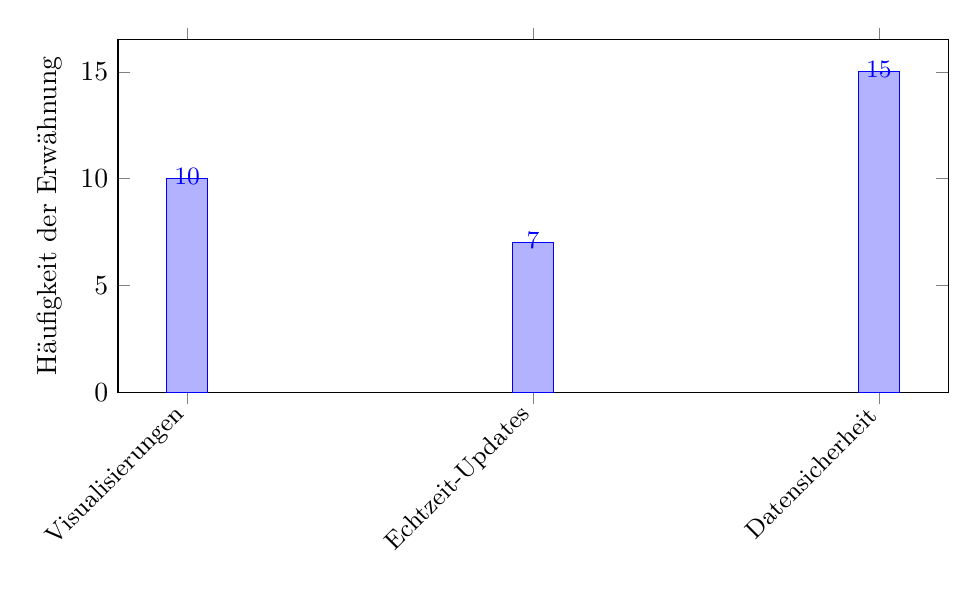
\begin{tikzpicture}
        \begin{axis}[
            width=\textwidth,
            height=0.5\textwidth,
            ybar,
            bar width=15pt,
            ylabel={Häufigkeit der Erwähnung},
            symbolic x coords={Visualisierungen, Echtzeit-Updates, Datensicherheit},
            xtick=data,
            x tick label style={font=\small, rotate=45, anchor=east},
            ymin=0,
            nodes near coords,
            nodes near coords style={font=\small, anchor=mid},
        ]
        \addplot coordinates {(Visualisierungen,10) (Echtzeit-Updates,7) (Datensicherheit,15)};
        \end{axis}
    \end{tikzpicture}
    \caption{Häufigkeit genannter Anforderungen aus Stakeholder-Interviews.}
    \label{fig:stakeholder_results_barchart}
\end{figure}
\newpage

\section{Vergleich bestehender Lösungen}
\subsection{Vergleich von HRworks und Evalea}
Die bestehenden Tools HRworks und Evalea wurden hinsichtlich ihrer Funktionen analysiert.

\begin{table}[h!]
\centering
\caption{Vergleich von HRworks und Evalea}
\label{tab:vergleich_hrworks_evalea}
\begin{tabularx}{\textwidth}{|X|X|X|}
\hline
\textbf{Kriterium}              & \textbf{HRworks}                                                                 & \textbf{Evalea}                                                                 \\\hline
Visualisierung                  & Keine spezialisierte Visualisierung.                                            & Umfangreiche Reporting-Funktionen.                                             \\\hline
Datenmanagement                 & Basis-Stammdatenverwaltung.                                                     & Strukturierte Verwaltung mit erweiterten Reporting-Optionen.                   \\\hline
Feedback                        & 360°-Feedback-Funktionen.                                                      & Anpassbare Gesprächsleitfäden.                                                 \\\hline
Benutzerfreundlichkeit          & Intuitive Bedienung.                                                           & Flexible Konfigurationsmöglichkeiten.                                          \\\hline
Integration                     & Fokus auf allgemeine HR-Prozesse.                                              & Nahtlose Integration in bestehende Systeme.                                    \\\hline
\end{tabularx}
\end{table}

\begin{figure}[h!]
    \centering
    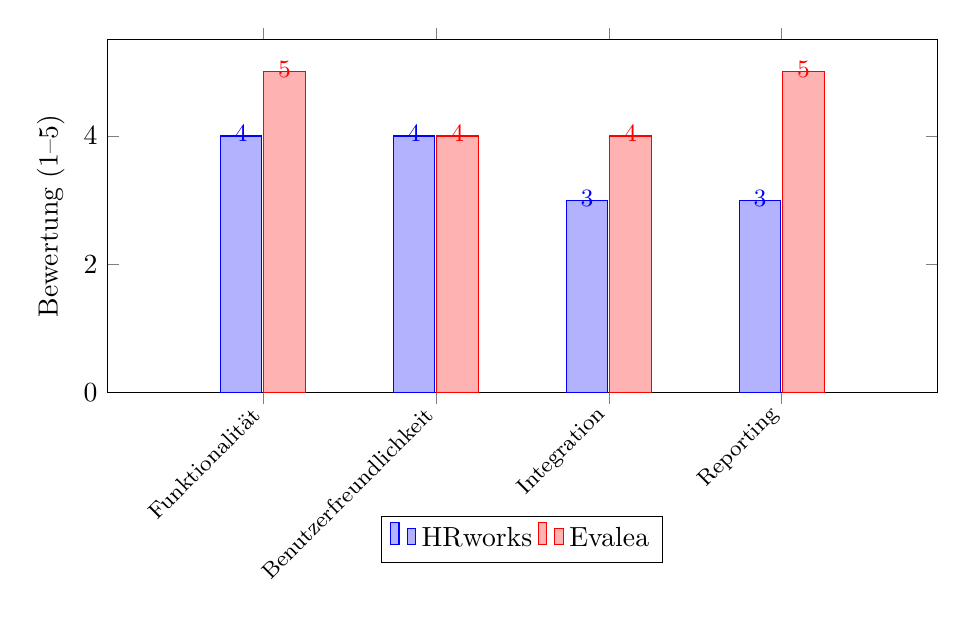
\begin{tikzpicture}
        \begin{axis}[
            width=\textwidth,
            height=0.5\textwidth,
            ybar=0.7pt,
            bar width=15pt,
            enlarge x limits=0.3,
            ylabel={Bewertung (1–5)},
            symbolic x coords={Funktionalität, Benutzerfreundlichkeit, Integration, Reporting},
            xtick=data,
            x tick label style={font=\footnotesize, rotate=45, anchor=east},
            ymin=0, ymax=5.5,
            nodes near coords,
            nodes near coords style={font=\small, anchor=mid},
            legend style={at={(0.5,-0.35)}, anchor=north, legend columns=-1},
            legend cell align={left}
        ]
        \addplot[blue,fill=blue!30] coordinates {
            (Funktionalität,4)
            (Benutzerfreundlichkeit,4)
            (Integration,3)
            (Reporting,3)
        };
        \addplot[red,fill=red!30] coordinates {
            (Funktionalität,5)
            (Benutzerfreundlichkeit,4)
            (Integration,4)
            (Reporting,5)
        };
        \legend{HRworks, Evalea}
        \end{axis}
    \end{tikzpicture}
    \caption{Vergleich zwischen HRworks und Evalea in verschiedenen Kategorien.}
    \label{fig:hrworks_evalea_comparison}
\end{figure}
